\section{Data Understanding and Preparation}
The dataset contains 32 columns and 149531 rows of titles of different types.
For each title, the dataset contains information regarding many different
aspects. Table~\ref{tab:initial_categorical_features} lists the initial categorical
features.
\begin{table}[H]
    \centering
    \begin{tabular}{|p{4cm}|p{9cm}|}

        \hline
        \textbf{Feature} & \textbf{Description} \\ \hline
        % Categorical
        \texttt{originalTitle} & Original title, in the original language (?) \\ \hline
        \texttt{isAdult} & Whether or not the title is for adult \\ \hline
        \texttt{canHaveEpisodes} & Whether the title can have episodes \\ \hline
        \texttt{isRatable} & Whether the title can be rated by users \\ \hline
        \texttt{titleType} & Type of the title (e.g., movie, tvseries) \\ \hline
        \texttt{countryOfOrigin} & Countries where the title was primarily produced \\ \hline
        \texttt{genres} & Genres associated with the title \\ \hline
        \texttt{regions} & Regions for this version of the title \\ \hline
        \texttt{soundMixes} & Technical specification of sound mixes \\ \hline
        % Ordinal
        \texttt{worstRating} (ordinal) & Worst title rating \\ \hline
        \texttt{bestRating} (ordinal) & Best title rating \\ \hline
        \texttt{rating} (ordinal) & IMDB title rating class \\ \hline
    \end{tabular}
    \caption{Initial categorical features of the IMDb dataset}
    \label{tab:initial_categorical_features}
\end{table}


Of the initial categorical attributes, the following were removed:
\begin{itemize}
    \item \texttt{originalTitle}, as it did not provide particularly useful
    information;
    \item \texttt{isAdult}, as it was almost completely correlated with the
    \textit{Adult} genre, so a logical OR operation was performed, and the genre
    only was kept;
    \item \texttt{canHaveEpisodes}, as it was completely correlated with the title type
    being \textit{tvSeries} or \textit{tvMiniSeries};
    \item \texttt{isRatable}, as it was always true;
    \item \texttt{soundMixes}, as it required some domain knowledge to be understood, as well as having issues with the values it contained.
    \item \texttt{worstRating} and \texttt{bestRating}, as they were always
    1 and 10, respectively;
    \item \texttt{rating}, as it was obtainable from the \texttt{averageRating}
    continuous attribute, through a simple discretization.
\end{itemize}


Table~\ref{tab:initial_features_numerical} lists the initial numerical features.


\begin{table}[H]
    \centering
    \begin{tabular}{|p{4cm}|p{9cm}|}
        \hline
        \textbf{Feature} & \textbf{Description} \\ \hline
        % Continuous
        \texttt{startYear} & Release year of the title (series start year for TV) \\ \hline
        \texttt{endYear} & TV Series end year \\ \hline
        \texttt{runtimeMinutes} & Primary runtime of the title, in minutes \\ \hline
        \texttt{numVotes} & Number of votes the title has received \\ \hline
        \texttt{numRegions} & Number of regions for this version of the title \\ \hline
        \texttt{totalImages} & Total number of images for the title \\ \hline
        \texttt{totalVideos} & Total number of videos for the title \\ \hline
        \texttt{totalCredits} & Total number of credits for the title \\ \hline
        \texttt{criticReviewsTotal} & Total number of critic reviews \\ \hline
        \texttt{awardWins} & Number of awards the title won \\ \hline
        \texttt{awardNominations} & Number of award nominations excluding wins \\ \hline
        \texttt{ratingCount} & Total number of user ratings submitted \\ \hline
        \texttt{userReviewsTotal} & Total number of user reviews \\ \hline
        \texttt{castNumber} & Total number of cast individuals \\ \hline
        \texttt{CompaniesNumber} & Total number of companies that worked for the title \\ \hline
        \texttt{averageRating} & Weighted average of all user ratings \\ \hline
        \texttt{externalLinks} & Total number of external links on IMDb page \\ \hline
        \texttt{quotesTotal} & Total number of quotes on IMDb page \\ \hline
        \texttt{writerCredits} & Total number of writer credits \\ \hline
        \texttt{directorCredits} & Total number of director credits \\ \hline
    \end{tabular}
    \caption{Initial numerical features of the IMDb dataset}
    \label{tab:initial_features_numerical}
\end{table}

Of the initial numerical attributes, the following were removed:
\begin{itemize}
    \item \texttt{endYear}, as it had no values for non-Series titles, and having around 50\% of missing values for \textit{tvSeries} and
\textit{tvMiniSeries};
    \item \texttt{numVotes}, as it had a very high correlation with \texttt{ratingCount};
\end{itemize}

Figure~\ref{fig:skewness} shows the skewness of some of the numerical features.
It can be observed that many features exhibit a heavy right skew, with a long tail of high values.

    
Figure~\ref{fig:rating_dist} shows the distribution of the
\texttt{averageRating} attribute.
\begin{figure}[H]
    \centering
    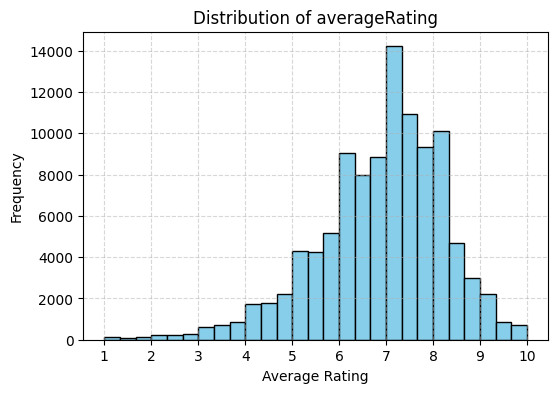
\includegraphics[width=0.6\textwidth]{plotsss/rating_distrib.png}
    \caption{Distribution of the \texttt{averageRating} attribute}
    \label{fig:rating_dist}
\end{figure}
The distribution is Normal-like, with a peak around 7.
This graph is particularly important because of the centrality
of the feature in the classification and regression tasks.

\subsection{Feature Engineering}
\begin{itemize}
    \item \texttt{totalImages}, \texttt{totalVideos} and \texttt{quotesTotal}, were merged
through a simple sum operation
into a single feature (\texttt{totalMedia}) because of their similar semantic
meaning, as well as heavy right skewness;
    \item \texttt{awardWins} and \texttt{awardNominations}, were merged with the same procedure
as above into \texttt{totalNominations}, since they represented the same concept;
    \item \texttt{userReviewsTotal} and\texttt{criticReviewsTotal},were merged with the same procedure
as above into \texttt{reviewsTotal}, since they represented the same concept;
    \item \texttt{regions} and \texttt{countryOfOrigin},
were merged through a simple union operation. The resulting feature was then
represented trhough frequency encoding on the entire list, as well as
counts of the number of countries from each continent.
This resulted in eight new features (six continents, one for unknown country codes,
and the last for the frequency encoding);
    \item \texttt{genre}, it was observed that each record
contained up to three genres, listed in alphabetical order—indicating that the order
did not convey any semantic information about the title.
To represent this information, three separate features were created, each
corresponding to one of the genres. These features were encoded using frequency
encoding, sorted in descending order of frequency across the dataset.  
A value of 0 was used to indicate missing genres—either when no genres were present or
to fill the remaining slots when fewer than three were available;
\item \texttt{titleType}, was one-hot encoded, as it was a nominal categorical
feature with no intrinsic order;
    \item \texttt{deltaCredits}, was created as the difference between
\texttt{totalCredits} and the sum of \texttt{castNumber}, \texttt{writerCredits} and \texttt{directorCredits}. 
This feature aimed to capture the number of other types of credits
(such as producers, editors, etc.) associated with a title, which could be relevant for
understanding its production scale and complexity;
    \item \texttt{runtimeMinutes}, had a very high number of missing values approx ~27\%. 
    Since the feature had high relevance in the domain, it was
imputed with the interquartile range, separately for each title
type. For advanced classification, in order to avoid any correlation with the target variable, 
we imputed the feature with random integers within the global interquartile range.

\end{itemize}



